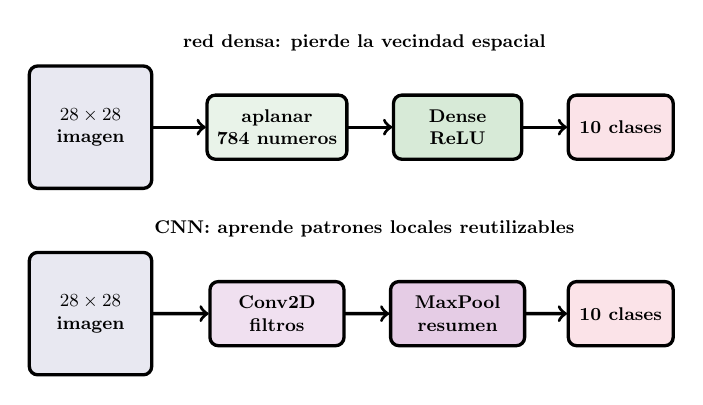
\begin{tikzpicture}[scale=0.74,transform shape]
\tikzstyle{box}=[draw,rounded corners=3pt,very thick,align=center,font=\small\bfseries]

\node[box,fill=MidnightBlue!10,minimum width=2.1cm,minimum height=2.1cm] (img1) at (0,0) {$28\times28$\\imagen};
\node[box,fill=ForestGreen!10,minimum width=2.4cm,minimum height=1.1cm] (flat) at (3.2,0) {aplanar\\784 numeros};
\node[box,fill=ForestGreen!18,minimum width=2.2cm,minimum height=1.1cm] (dense) at (6.3,0) {Dense\\ReLU};
\node[box,fill=Crimson!12,minimum width=1.8cm,minimum height=1.1cm] (out1) at (9.1,0) {10 clases};
\draw[->,very thick] (img1) -- (flat);
\draw[->,very thick] (flat) -- (dense);
\draw[->,very thick] (dense) -- (out1);
\node[font=\small\bfseries] at (4.7,1.45) {red densa: pierde la vecindad espacial};

\node[box,fill=MidnightBlue!10,minimum width=2.1cm,minimum height=2.1cm] (img2) at (0,-3.2) {$28\times28$\\imagen};
\node[box,fill=Purple!12,minimum width=2.3cm,minimum height=1.1cm] (conv) at (3.2,-3.2) {Conv2D\\filtros};
\node[box,fill=Purple!20,minimum width=2.3cm,minimum height=1.1cm] (pool) at (6.3,-3.2) {MaxPool\\resumen};
\node[box,fill=Crimson!12,minimum width=1.8cm,minimum height=1.1cm] (out2) at (9.1,-3.2) {10 clases};
\draw[->,very thick] (img2) -- (conv);
\draw[->,very thick] (conv) -- (pool);
\draw[->,very thick] (pool) -- (out2);
\node[font=\small\bfseries] at (4.7,-1.75) {CNN: aprende patrones locales reutilizables};
\end{tikzpicture}
